\documentclass{beamer}
%%% ========== Package setup ==========
\usepackage{xeCJK}      % Chinese words package
\usepackage{fontspec}   % Word fonts package
\usepackage{listings}   % Wrap Figure or table package
\usepackage{wrapfig}    % Multicolumn package
\usepackage{multicol}   % Multicolumn package
\usepackage{pdflscape}  % Landscpae package
\usepackage{tikz}       % TikZ picture package(Docs: https://ftp.ntou.edu.tw/ctan/graphics/pgf/base/doc/pgfmanual.pdf)
\usepackage[outline]{contour} % glow around text
\usepackage{amsmath}
\usepackage{mathtools}

%%% ========== Slide setting ==========
%% Slide theme setup
\usetheme{CambridgeUS}
\usecolortheme{wolverine}

%% Setup chinese words encoder
\XeTeXlinebreaklocale "zh"
\XeTeXlinebreakskip = 0pt plus 1pt

%% More word fonts
\setmainfont{Times New Roman}
\renewcommand{\familydefault}{\rmdefault}
\setCJKmainfont{標楷體}

% Setting for figure and table numbering
\setbeamertemplate{caption}[numbered]

% TikZ setting
\usetikzlibrary{positioning}
\usetikzlibrary{calc}
\usetikzlibrary{arrows.meta}

%%% ========== Title setup ==========
\date{July 25, 2022}
\title{Meeting}
\author{Po Hsun Wu}

%%% ========== Document ==========
\begin{document}
    \maketitle

    \section{Progress report}
    \begin{frame}
        \frametitle{\secname}

        \begin{itemize}
            \item Fixed the simulation.
            \begin{figure}
                \centering
                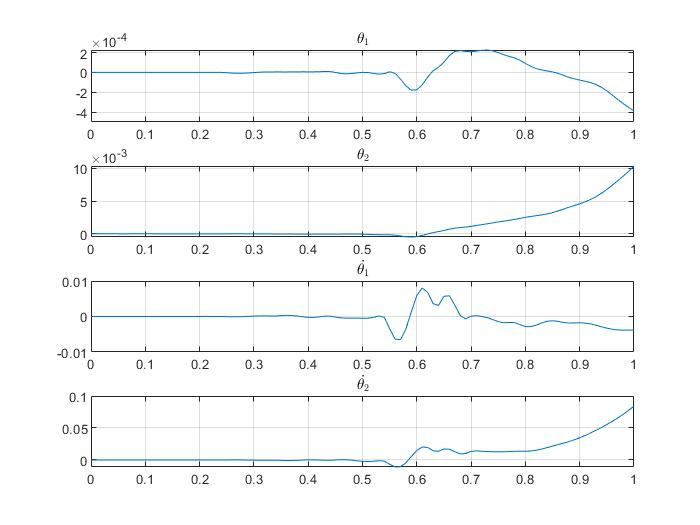
\includegraphics[scale=.3]{Figs/error.jpg}
                \caption{Error between python and ODE45}

            \end{figure}
        \end{itemize}
    \end{frame}

    \begin{frame}
        \frametitle{\secname}

        \begin{itemize}
            \item Train the controller using Q-learning method.
            \begin{figure}
                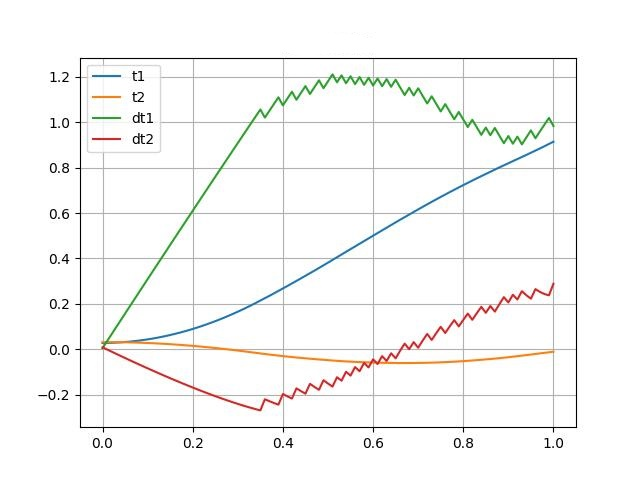
\includegraphics[scale=.3]{Figs/train2.jpg}
                \caption{Training result}
            \end{figure}
        \end{itemize}
    \end{frame}

    \section{Future}
    \begin{frame}
        \frametitle{\secname}

        \begin{itemize}
            \item Fix the reward system.
            \begin{figure}
                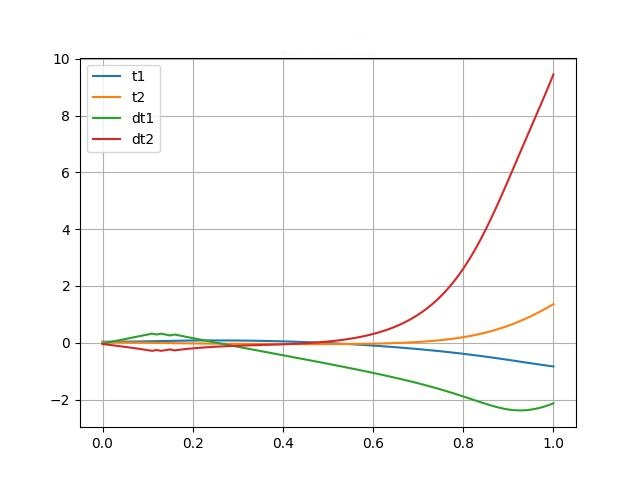
\includegraphics[scale=.3]{Figs/train1.jpg}
                \caption{Training result}
            \end{figure}
        \end{itemize}

    \end{frame}

\end{document}